\documentclass[12pt,a4paper]{article}
\usepackage[
	top=25mm,
	left=25mm,
	right=25mm,
	bottom=25mm,
	headheight=55pt,
	footskip   = 10pt,
]{geometry}
%\usepackage{t1enc}
\usepackage{lmodern} % pdflatex or dvi latex
\usepackage[T1]{fontenc}
\usepackage[utf8]{inputenc}

\usepackage{fontspec}
\setmainfont{Times New Roman}
%\setmainfont{Raleway-Regular}
\usepackage[mathscr]{eucal}
\usepackage[magyar]{babel}
\usepackage{amssymb}
\usepackage{amsthm}
\usepackage{graphics}
\usepackage{amsxtra}

%fejléc-----------------------------------------------------------------------

\usepackage{fancyhdr}
\usepackage[most]{tcolorbox}
\usepackage{color, colortbl}

\usepackage{setspace}
\usepackage{enumitem}    

%functions-----------------------------------------------------------------------
\DeclareMathOperator{\arccot}{arccot}
\DeclareMathOperator{\arctg}{arctg}
\DeclareMathOperator{\arcctg}{arcctg}
\DeclareMathOperator{\tg}{tg}
\DeclareMathOperator{\ctg}{ctg}

%colors------------------------------------------------------------------
\definecolor{PannonLightBlue}{RGB}{11,142,216}
\definecolor{PannonDarkBlue}{RGB}{2,34,55}

%checkbox, dotfill------------------------------------
\newcommand{\checkbox}{$\square$}
\newcommand\fillin[1][3cm]{\makebox[#1]{\dotfill}}
\newcommand\fillinlong[1][5.5cm]{\makebox[#1]{\dotfill}}
\newcommand\fillinshort[1][1cm]{\makebox[#1]{\dotfill}}




%header and footer---------------------------------------------
\fancypagestyle{first}{%
\fancyhf{}
\renewcommand{\headrulewidth}{1pt}
%\renewcommand{\headrule}{\hbox to\headwidth{\color{PannonDarkBlue}\leaders\hrule height \headrulewidth\hfill}}

\fancyhead[L]{%
%  \scshape
  \color{black}
Matematika\\
középszint}
\fancyhead[R]{%
%  \scshape
  \color{black}
Név: \fillinlong osztály: \fillinshort}

\renewcommand{\footrulewidth}{1pt}
%\fancyfoot[L]{\vspace{0.2cm}\includegraphics[scale=.2]{mp_presentation_logo}}
\fancyfoot[L]{\vspace{0.2cm}2211 írásbeli vizsga, I. összetevő} 
\fancyfoot[C]{\vspace{0.2cm} \thepage\hspace{2pt} / \hspace{2pt}\pageref{LastPage}}   
\fancyfoot[R]{\vspace{0.2cm}2022. október 18.}  
}

\fancypagestyle{second}{%
\setcounter{page}{1}
\fancyhf{}
\renewcommand{\headrulewidth}{1pt}
%\renewcommand{\headrule}{\hbox to\headwidth{\color{PannonDarkBlue}\leaders\hrule height \headrulewidth\hfill}}

\fancyhead[L]{%
%  \scshape
  \color{black}
Matematika\\
középszint}
\fancyhead[R]{%
%  \scshape
  \color{black}
Név: \fillinlong osztály: \fillinshort}

\renewcommand{\footrulewidth}{1pt}
%\fancyfoot[L]{\vspace{0.2cm}\includegraphics[scale=.2]{mp_presentation_logo}}
\fancyfoot[L]{\vspace{0.2cm}2211 írásbeli vizsga, II. összetevő} 
\fancyfoot[C]{\vspace{0.2cm} \thepage\hspace{2pt} / \hspace{2pt}\pageref{SecondLastPage}}   
\fancyfoot[R]{\vspace{0.2cm}2022. október 18.}  
}


\fancypagestyle{solution}{%
\setcounter{page}{1}
\fancyhf{}
\renewcommand{\headrulewidth}{1pt}
%\renewcommand{\headrule}{\hbox to\headwidth{\color{PannonDarkBlue}\leaders\hrule height \headrulewidth\hfill}}

\fancyhead[L]{%
%  \scshape
  \color{black}
Matematika - középszint}
\fancyhead[R]{%
%  \scshape
  \color{black}
Javítási-értékelési útmutató}

\renewcommand{\footrulewidth}{1pt}
%\fancyfoot[L]{\vspace{0.2cm}\includegraphics[scale=.2]{mp_presentation_logo}}
\fancyfoot[L]{\vspace{0.2cm}2211 írásbeli vizsga, Megoldás} 
\fancyfoot[C]{\vspace{0.2cm} \thepage\hspace{2pt} / \hspace{2pt}\pageref{SolutionLastPage}}   
\fancyfoot[R]{\vspace{0.2cm}2022. október 18.}  
}



\usepackage{pgfplots}
\usepackage{tikz}
%tikz library setup------------------------------------
\usetikzlibrary{arrows,positioning,shapes,fit,calc}
\usetikzlibrary{arrows.meta,shadings,bending}
\usetikzlibrary{shapes.geometric,positioning}
\usetikzlibrary{math, shapes.misc}
\usetikzlibrary{intersections}
\usetikzlibrary{backgrounds}
\usetikzlibrary{decorations.pathreplacing} 
\usepgfplotslibrary{fillbetween}
\usetikzlibrary{decorations.pathmorphing,shadows}
\usetikzlibrary{angles,quotes}

\pgfplotsset{compat=1.14}


\begin{document}
% I. összetevő------------------------------------

\pagestyle{first}
\begin{enumerate}[font=\bfseries]

  % 1. feladat------------------------------------
  \item
        \begin{spacing}{1.2}
          Adott a pozitív egész számok halmazának két részhalmaza:\\
          $A=\lbrace 12\text{-nél kisebb prímszámok} \rbrace$\\
          $B=\lbrace 3\text{-mal nem osztható egyjegyű számok} \rbrace$.\\
          Elemei felsorolásával adja meg az $A$, a $B$, az $A\cap B$ és a $B\setminus A$ halmazokat!
        \end{spacing}
        \vspace{3cm}
        \begin{flushright}
          \begin{tabular}{|m{5.5cm}| *3{>{\cellcolor{black!20}\centering\arraybackslash}m{1in}|} @{}m{0pt}@{}}
            \hline
            \begin{flushleft}
              $A=$
            \end{flushleft} & $1$ pont & \\[0ex]
            \hline
            \begin{flushleft}
              $B=$
            \end{flushleft} & $1$ pont & \\[0ex]
            \hline
            \begin{flushleft}
              $A\cap B=$
            \end{flushleft} & $1$ pont & \\[0ex]
            \hline
            \begin{flushleft}
              $B\setminus A=$
            \end{flushleft} & $1$ pont & \\[0ex]
            \hline
          \end{tabular}
        \end{flushright}

        % 2. feladat------------------------------------
  \item
        \begin{spacing}{1.2}
          Hány olyan háromjegyű pozitív egész szám van, melynek mindhárom számjegye nagyobb $5$-nél?
        \end{spacing}
        \vspace{2cm}
        \begin{flushright}
          \begin{tabular}{|m{5.5cm}| *3{>{\cellcolor{black!20}\centering\arraybackslash}m{1in}|} @{}m{0pt}@{}}
            \hline
            \begin{flushleft}

            \end{flushleft} & $2$ pont & \\[0ex]
            \hline
          \end{tabular}
        \end{flushright}

        % 3. feladat------------------------------------
  \item
        \begin{spacing}{1.2}
          Adja meg $n$ értékét úgy, hogy az alábbi egyenlőség igaz legyen!
          \begin{equation*}
            \dfrac{2^{7}\cdot 2^{6}}{2^{3}}=2^{n}
          \end{equation*}
        \end{spacing}
        \vspace{2cm}
        \begin{flushright}
          \begin{tabular}{|m{5.5cm}| *3{>{\cellcolor{black!20}\centering\arraybackslash}m{1in}|} @{}m{0pt}@{}}
            \hline
            \begin{flushleft}
              $n=$
            \end{flushleft} & $2$ pont & \\[0ex]
            \hline
          \end{tabular}
        \end{flushright}

        % 4. feladat------------------------------------
  \item
        \begin{spacing}{1.2}
          Egy $35$ g tömegű csokoládészelet csomagolásán az olvasható, hogy $100$ g termék $520$ kcal energiát tartalmaz. Hány kcal energiát tartalmaz ez a csokoládészelet?
        \end{spacing}
        \vspace{4cm}
        \begin{flushright}
          \begin{tabular}{|m{5.5cm}| *3{>{\cellcolor{black!20}\centering\arraybackslash}m{1in}|} @{}m{0pt}@{}}
            \hline
            \begin{flushleft}

            \end{flushleft} & $2$ pont & \\[0ex]
            \hline
          \end{tabular}
        \end{flushright}

        % 5. feladat------------------------------------
  \item
        \begin{spacing}{1.2}
          Az alábbi ábrán a $\left[−3; 2\right]$ zárt intervallumon értelmezett $x\mapsto -\left(x+1\right)^{2}+5$ függvény grafikonja látható. Adja meg a függvény értékkészletét és maximumának helyét!
        \end{spacing}
        \begin{center}
          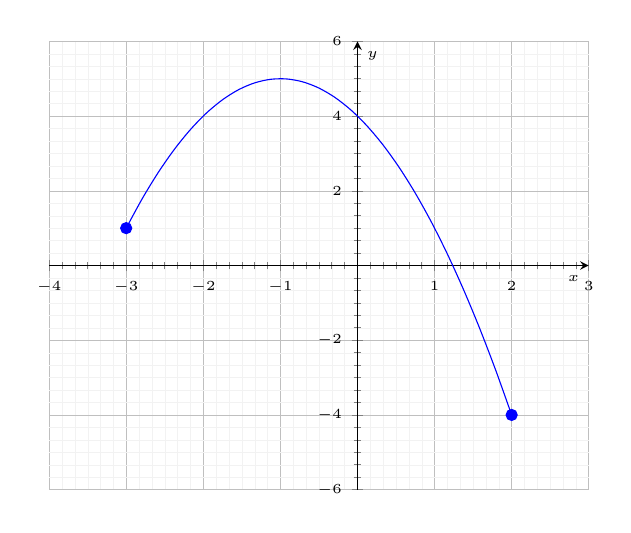
\begin{tikzpicture}
            \begin{axis}[
                xmin=-3.5,xmax=2.5,
                ymin=-5.5,ymax=5.5,
                grid=both,
                grid style={line width=.1pt, draw=gray!10},
                major grid style={line width=.2pt,draw=gray!50},
                axis lines=middle,
                inner axis line style={=>},
                minor tick num=5,
                enlargelimits={abs=0.5},
                %    axis line style={latex-latex},
                ticklabel style={font=\tiny},
                xlabel style={at={(ticklabel* cs:1)},anchor=north east},
                ylabel style={at={(ticklabel* cs:1)},anchor=north west},
                xlabel={\tiny $x$},
                ylabel={\tiny $y$}
              ]
              \addplot[blue,domain={-3:2},smooth] {-(x+1)^2+5} ;
              \addplot[blue, mark=*, only marks] coordinates {(-3,1) (2,-4)};
            \end{axis}

          \end{tikzpicture}
        \end{center}

        \vspace{4.5cm}
        \begin{flushright}
          \begin{tabular}{|m{5.5cm}| *3{>{\cellcolor{black!20}\centering\arraybackslash}m{1in}|} @{}m{0pt}@{}}
            \hline
            \begin{flushleft}
              Értékkészlet:
            \end{flushleft} & $2$ pont & \\[0ex]
            \hline
            \begin{flushleft}
              A maximum helye:
            \end{flushleft} & $1$ pont & \\[0ex]
            \hline
          \end{tabular}
        \end{flushright}

        % 6. feladat------------------------------------
  \item
        \begin{spacing}{1.2}
          Adja meg egy konvex nyolcszög átlóinak számát!
        \end{spacing}

        % 7. feladat------------------------------------
  \item

        % 8. feladat------------------------------------
  \item

        % 9. feladat------------------------------------
  \item

        % 10. feladat------------------------------------
  \item
        \begin{spacing}{1.2}
          Számítsa ki az alábbi háromszögben a $30^{\circ}$-os szöggel szemközti oldal hosszát!
          Megoldását részletezze!
        \end{spacing}

        \centering{
          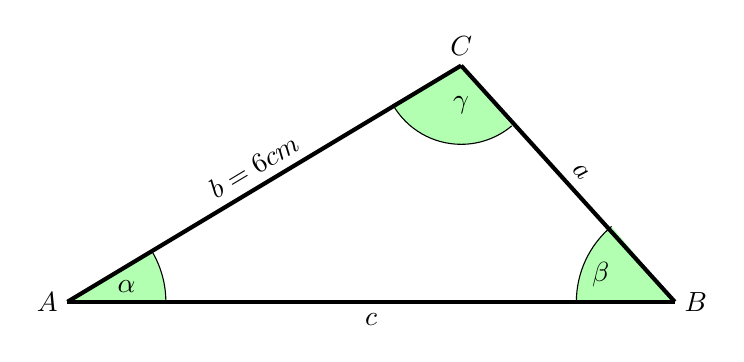
\begin{tikzpicture}
            \coordinate[label=left:$A$]  (A) at (0,0);
            \coordinate[label=right:$B$] (B) at (7.7135,0);
            \coordinate[label=above:$C$] (C) at (5,3);

            % angle alpha
            \draw[fill=green!30] (0,0) -- (0:1.25cm) arc (0:30:1.25cm);
            \draw (0.75cm,0.2cm) node {$\alpha$};

            % angle beta
            \begin{scope}[shift={(7.7135cm,0cm)}]
              \draw[fill=green!30] (0,0) -- (-180:1.25cm) arc (180:130:1.25cm);
              \draw (160:1cm) node {$\beta$};
            \end{scope}

            % angle gamma
            \begin{scope}[shift={(5cm,3cm)}]
              \draw[fill=green!30] (0,0) -- (-150:1cm) arc (-150:-50:1cm);
              \draw (-90:0.5cm) node {$\gamma$};
            \end{scope}

            % the triangle
            \draw [line width=1.5pt] (A) -- (C) node[above,midway,sloped] {$b=6cm$};
            \draw [line width=1.5pt] (A) -- (B)  node[below,midway,sloped] {$c$};
            \draw [line width=1.5pt] (B) -- (C)  node[above,midway,sloped] {$a$};
          \end{tikzpicture}
        }
        \vspace{5cm}
        \begin{flushright}
          \begin{tabular}{|m{5.5cm}| *3{>{\cellcolor{black!20}\centering\arraybackslash}m{1in}|} @{}m{0pt}@{}}
            \hline
            \begin{flushleft}
              Indoklásért járó pont
            \end{flushleft} & $2$ pont & \\[0ex]
            \hline
            \begin{flushleft}
              $a=$
            \end{flushleft} & $1$ pont & \\[0ex]
            \hline
          \end{tabular}
        \end{flushright}
\end{enumerate}


\label{LastPage}~

% II. összetevő------------------------------------

\newpage


\pagestyle{second}

\label{SecondLastPage}~

% Megoldás------------------------------------

\newpage


\pagestyle{solution}

\label{SolutionLastPage}~
\end{document}